\begin{surferPage}[Singularidad A3--]{Una singularidad $A_3^{--}$}
Mirando la ecuación
    \[x^4-y^2-z^2=0\]
se ve que esta superficie es similar a la anterior
(una $A_3^{+-}$, con ecuación $x^4+y^2-z^2$).
La imagen abajo a la izquierda muestra las dos superficies,
$A_3^{--}$ de color amarillo y $A_3^{+-}$ de color azul.
La sección con el plano $y=0$ da la misma curva en los dos casos:
    \vspace*{-0.5em}
    \begin{center}
      \begin{tabular}{c@{\qquad}c}
        \begin{tabular}{@{}c@{}}
          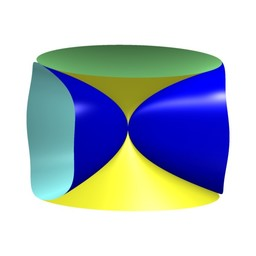
\includegraphics[width=1.6cm]{../../common/images/A3pmA3mm}
        \end{tabular}
        &
        \begin{tabular}{@{}c@{}}
          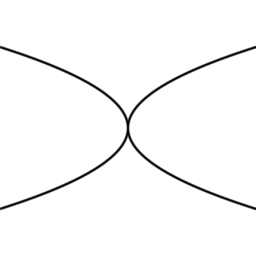
\includegraphics[width=1.6cm]{../../common/images/A3pm_cut}
        \end{tabular}
      \end{tabular}
    \end{center}
    \vspace*{-0.1cm}
Esta singularidad $A_3^{- -}$ también se puede deformar en
$2=\lfloor\frac{3+1}{2}\rfloor$ singularidades cónicas:
    %
    \begin{center}
      \vspace*{-0.1cm}
      \begin{tabular}{@{}c@{\quad}c@{\quad}c@{}}
        \begin{tabular}{@{}c@{}}
          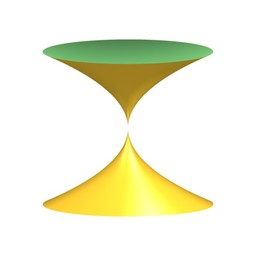
\includegraphics[width=1.6cm]{../../common/images/A3mm_0}
        \end{tabular}
        &
        \begin{tabular}{@{}c@{}}
          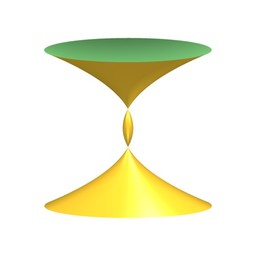
\includegraphics[width=1.6cm]{../../common/images/A3mm_1}
        \end{tabular}
        &
        \begin{tabular}{@{}c@{}}
          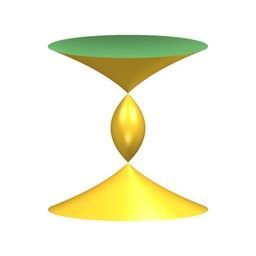
\includegraphics[width=1.6cm]{../../common/images/A3mm_2}
        \end{tabular}
      \end{tabular}
    \end{center}
    \vspace*{-0.2cm}
La deformación de $A_3^{--}$ mostrada en la imagen
es la dada por la siguiente ecuación:
    \[\bigl(x-\frac12 a^2\bigr)^2\bigl(x+\frac12 a^2\bigr)^2-y^2-z^2.\]
 
\end{surferPage}
